\documentclass[aspectratio=169]{beamer}
\usefonttheme[onlymath]{serif}
\usepackage[utf8]{inputenc}
\usepackage{graphicx} % Allows including images
\usepackage{booktabs} % Allows the use of \toprule, \midrule and \bottomrule in tables
\usepackage{subfigure}
\usepackage{subfiles}
\usepackage{url}
\usepackage{amssymb}
\usepackage{amsmath}
\usepackage{xcolor,colortbl}
\usepackage[backend=bibtex,sorting=none]{biblatex}
\usepackage[AutoFakeBold, AutoFakeSlant]{xeCJK}

\renewcommand{\figurename}{图}

\addbibresource{reference.bib} %BibTeX数据文件及位置

\definecolor{NJUPurple}{rgb}{0.41568, 0, 0.37255} 
\colorlet{LightNJUPurple}{white!60!NJUPurple}
\colorlet{SuperLightNJUPurple}{white!90!NJUPurple}

\addbibresource{reference.bib} %BibTeX数据文件及位置

\definecolor{NJUPurple}{rgb}{0.41568, 0, 0.37255} % UBC Blue (primary)

\usecolortheme[named=NJUPurple]{structure}

%Information to be included in the title page:
\title{基于模型的迁移学习}
\author{\href{mailto:}{田鸿龙}}
\institute{LAMDA, Nanjing University}
\date{\today}

%Logo in every slide
\logo{%
  \makebox[0.98\paperwidth]{
    \href{https://www.nju.edu.cn}{
\includegraphics[height=0.75cm,keepaspectratio]{logos/nju_logo.jpg}}
    \hfill%
    \href{https://www.lamda.nju.edu.cn}{
\includegraphics[height=0.75cm,keepaspectratio]{logos/lamda_logo.png}}%
  }
}

\setbeamertemplate{blocks}[rounded][shadow=true]
\setbeamercolor{block title}{fg=white,bg=NJUPurple!50}
\setbeamercolor{block body}{fg=black,bg=white}
\setbeamerfont{title}{shape=\bfseries,size=\Large}
\setbeamerfont{author}{shape=\bfseries}

\makeatletter
\setbeamertemplate{title page}{%
  \vbox{}
  \vfill
  \vskip2cm%<- added
  \begingroup
    \centering
    \begin{beamercolorbox}[sep=8pt,center]{title}
      \usebeamerfont{title}\inserttitle\par%
      \ifx\insertsubtitle\@empty%
      \else%
        \vskip0.25em%
        {\usebeamerfont{subtitle}\usebeamercolor[fg]{subtitle}\insertsubtitle\par}%
      \fi%     
    \end{beamercolorbox}%
    \vskip1em\par
    \vfill%<- added
    \begin{beamercolorbox}[sep=8pt,center]{author}
      \usebeamerfont{author}\insertauthor
    \end{beamercolorbox}
    \vskip-0.2cm%<- changed
    \begin{beamercolorbox}[sep=8pt,center]{institute}
      \usebeamerfont{institute}\insertinstitute
    \end{beamercolorbox}
    \vfill%<- added
    \begin{beamercolorbox}[sep=8pt,center]{date}
      \usebeamerfont{date}\insertdate
    \end{beamercolorbox}%
    \vskip0.5cm%<- changed
  \endgroup
%  \vfill%<- removed
}
\makeatother


%Contents before every section's starting slide
% https://tex.stackexchange.com/questions/193975/highlight-only-current-subsection-hide-subsections-of-other-sections
\AtBeginSection[]
{
  \begin{frame}
    \frametitle{目录}
  \tableofcontents[
        currentsection,
        currentsubsection,
        subsectionstyle=show/show/hide,
        sectionstyle=show/shaded
    ]
  \end{frame}
}

\AtBeginSubsection[]
{
  \begin{frame}
    \frametitle{目录}
  \tableofcontents[
        currentsection,
        currentsubsection,
        sectionstyle=show/shaded,
        subsectionstyle=show/shaded/hide,
    ]
  \end{frame}
}
% shape, colour of item, nested item bullets in itemize only
\setbeamertemplate{itemize item}[circle] \setbeamercolor{itemize item}{fg=NJUPurple}
\setbeamertemplate{itemize subitem}[circle] \setbeamercolor{itemize subitem}{fg=LightNJUPurple}
\setbeamertemplate{itemize subsubitem}[circle] \setbeamercolor{itemize subsubitem}{fg=SuperLightNJUPurple}
% font size of nested and nested-within-nested bulltes in both itemize and enumerate
% options are \tiny, \small, \scriptsize, \normalsize, \footnotesize, \large, \Large, \LARGE, \huge and \Huge


\setbeamerfont{itemize/enumerate subbody}{size=\scriptsize} 
\setbeamerfont{itemize/enumerate subsubbody}{size=\scriptsize}

%%setting up some useful slide creation commands
%split slide
\newenvironment{splitframe}[5]
%[1] ==> 1 parameter passed through {}
%[2] ==> 2 parameters passed through {}{}
%[4] ==> 4 parameters passed through {}{}{}{}
    {
    \begin{frame}{#3}
    \begin{columns}
    \column{#1\linewidth}
    \centering
    #4
    \column{#2\linewidth}
    \centering
    #5
    \end{columns}
    \centering
    \vspace{\baselineskip} % adds one line space
    }
    %Inside the first pair of braces (ABOVE) is set what your new environment will do before the text within, then inside the second pair of braces (BELOW) declare what your new environment will do after the text. Note second pair can be empty braces too.
    {
    \end{frame}
    }

\begin{document}

\frame{\titlepage}

% no hyperlinks in logos except for titlepage
\logo{%
  \makebox[0.98\paperwidth]{
    
\includegraphics[height=0.75cm,keepaspectratio]{logos/nju_logo.jpg}
    \hfill%
    
\includegraphics[height=0.75cm,keepaspectratio]{logos/lamda_logo.png}%
  }
}

\section{引言}
\begin{frame}
  \frametitle{基于模型的迁移学习}
  核心思想:在模型层次上原任务和目标任务共享部分通用知识。
  \begin{figure}
    \centering
    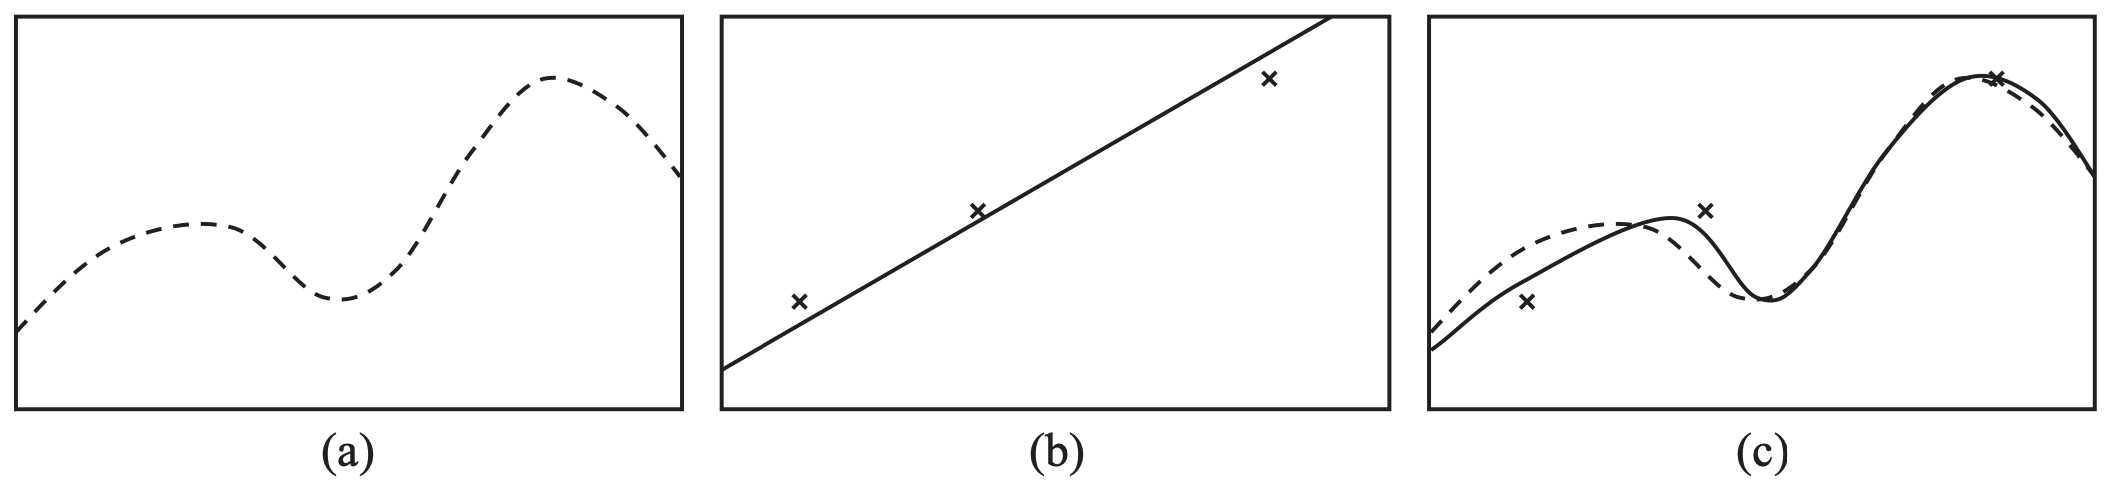
\includegraphics[width=0.8\textwidth]{imgs/model_based_TL.png}
  \end{figure}
  
  \begin{itemize}
    \item [(a)]Source model (the dash line)
    \item [(b)] Target model (the solid line) only with limited target data (the crosses)
    \item [(c)] The target model (the solid line) trans-ferred with the source model (the dash line) as a prior.

  \end{itemize}
\end{frame}

\begin{frame}
  \frametitle{基于模型的迁移学习和多任务学习}
  相同点
  \begin{itemize}
    \item 都是通过模型共享知识
    \item 往往可以通过调整多任务学习算法得到对应的迁移学习算法
  \end{itemize}
  不同点
  \begin{itemize}
    \item 多任务学习是同时训练的,而迁移学习具有顺序性
    \item 多任务学习要求算法在多个任务上表现良好,而迁移学习只关注\textbf{目标任务}
    \item 多任务学习无法达到单个任务的最优,而迁移学习要求在\textbf{目标任务}上达到最优
  \end{itemize}
\end{frame}

\begin{frame}
  \frametitle{分类}

  \begin{itemize}
    \item 基于共享模型成分的迁移学习
    \item 基于正则化的迁移学习
  \end{itemize}

\end{frame}

\section{基于共享模型成分的迁移学习}
\subsection{利用高斯过程的迁移学习}

\begin{frame}
  \frametitle{统计学习中的回归问题定义}
  \begin{itemize}
    \item 对于每个输入$\mathbf{x}$,对应一个输出$y$,通过数据集$\mathbf{X}=\left[\mathbf{x}_{1}, \mathbf{x}_{2}, \ldots, \mathbf{x}_{N}\right]^{T}$,$\mathbf{y}=\left[y_{1}, y_{2}, \ldots, y_{N}\right]^{T}$学习一个映射函数。
    \item $y$往往是含有噪声的,也就是说我们的数据集并不完全准确,定义潜变量$z$为$\mathbf{x}$对应的输出,我们的目标其实是学习映射函数$f:\mathbf{x} \rightarrow z$
    \item 根据数据集$\mathbf{X}$和$\mathbf{y}$得不到$f:\mathbf{x} \rightarrow z$的有效信息,我们假定$p(y\mid z) = N(z,\beta ^{-1})$
    \item 其中$\beta$表示精度,它的倒数$\beta ^{-1}$表示方差,$\beta$可以被学习得到。
  \end{itemize}
\end{frame}

\begin{frame}
  \frametitle{高斯过程回归}
  回归就是给一堆已知的$\mathbf{x}$和$y$,然后当拿出一个新$\mathbf{x}$的时候,能够预测出对应的$y$。高斯过程是一种贝叶斯方法,能够预测出新的$y$的分布来。

  高斯过程的出发点就是,如果两个$\mathbf{x}$比较近,那么对应的$y$一定是比较接近。给出的新$\mathbf{x}$,就看这个新的$\mathbf{x}$与之前给出的一堆$\mathbf{x}$有多近,从而知道新的$y$与之前的一堆$y$有多近,从而预测新$y$的值。
  
  基于上面的出发点,高斯过程回归要解决的问题如下:
  \begin{itemize}
    \item 如何度量$\mathbf{x}$之间有多近
    \item $\mathbf{x}$的“近”又如何反应到$y$有多近
  \end{itemize}
\end{frame}

\begin{frame}
  \frametitle{高斯过程回归(cont.)}
  高斯先验
  $$
  p(\mathbf{z} \mid \mathbf{X}, \theta)=N(\mathbf{0}, \mathbf{K})
  $$
  \begin{itemize}
    \item 高斯先验只和数据集中的$\mathbf{X}$有关
    \item $\mathbf{K}$是$\mathbf{X}$的相关系数(协方差矩阵),在这里相关系数用Kernel表示(假设有$N$个样本,则Kernel是$N \times N$的矩阵,和传统意义上的协方差矩阵不同,见下页Slide)
    \item 可以理解为,在算法没有“看到”$y$时,根据$\mathbf{X}$对$y$的相关性的假设
    \item 因为算法没有“看到”$y$,高斯分布的均值设为0
  \end{itemize}
\end{frame}

\begin{frame}
  \frametitle{高斯过程回归(cont.)}
  Kernel
  $$
  K(\mathbf{x},\mathbf{x}^{\prime} )=\sigma^{2} \exp \left(-\frac{\left\|\mathbf{x}-\mathbf{x}^{\prime}\right\|^{2}}{2 \ell^{2}}\right)
  $$
  \begin{itemize}
    \item 上述(书中)使用的Kernel是高斯核,实际上不限于此
    \item Kernel用来表示两个向量$\mathbf{x}$和$\mathbf{x}^{\prime}$的某些关系,高斯核往往用来描述两个向量有多“近”
    \item Kernel实际上可以看作向量$\mathbf{x}$在某个映射下的协方差矩阵
  \end{itemize}
\end{frame}

\begin{frame}
  \frametitle{高斯过程回归(cont.)}
  $$
  p(\mathbf{y}) = \int p(\mathbf{y}\mid \mathbf{z})p(\mathbf{z}) \mathrm{d}{\mathbf{z}} = N(\mathbf{y} \mid \mathbf{0}, \mathbf{C})
  $$

  $$
  C\left(\mathbf{x}_{n}, \mathbf{x}_{m}\right)=k\left(\mathbf{x}_{n}, \mathbf{x}_{m}\right)+\beta^{-1} \delta_{n m}
  $$

  用$\mathbf{y_N}$表示原来的数据集(训练集),用$\mathbf{y_{N+1}}$表示训练集和测试集的并集(不是一般性,假设测试集只有一个样本)
  $$
  p(y_{N + 1}) = \frac{p(\mathbf{y}_{N+1})}{p(\mathbf{y}_N)}
  $$
\end{frame}

\begin{frame}
  \frametitle{高斯过程回归(cont.)}
  $$
  p\left(\mathbf{y}_{N+1}\right)=\mathcal{N}\left(\mathbf{y}_{N+1} \mid \mathbf{0}, \mathbf{C}_{N+1}\right)
  $$
  其中
  $$
  \mathbf{C}_{N+1}=\left(\begin{array}{cc}
  \mathbf{C}_{N} & \mathbf{k} \\
  \mathbf{k}^{\mathrm{T}} & c
  \end{array}\right)
  $$
  $\mathbf{k}$ has elements $k(\mathbf{x}_n,\mathbf{x}_{N+1})$ and $n = 1,\cdots,N$, $c=k\left(\mathbf{x}_{N+1}, \mathbf{x}_{N+1}\right)+\beta^{-1}$
  \\最后
  $$p(y_{N+1} \mid \mathbf{y}_{N}) = N(m\left(\mathbf{x}_{N+1}\right), \sigma^{2}\left(\mathbf{x}_{N+1}\right))$$
  
  其中
  $$\begin{aligned} m\left(\mathbf{x}_{N+1}\right) &=\mathbf{k}^{\mathrm{T}} \mathbf{C}_{N}^{-1} \mathbf{t} \\ \sigma^{2}\left(\mathbf{x}_{N+1}\right) &=c-\mathbf{k}^{\mathrm{T}} \mathbf{C}_{N}^{-1} \mathbf{k} \end{aligned}$$
\end{frame}

\begin{frame}
  \frametitle{多任务高斯过程}
  设多个任务对应的任务集为$\left\{\left(\mathbf{X}_{m}, \mathbf{y}_{m}\right)\right\}$,联合概率分布$\mathbf{y}=\left(\mathbf{y}_{1}^{T}, \ldots, \mathbf{y}_{M}^{T}\right)^{T}$的概率为
  $$p(\mathbf{y} \mid \mathbf{X}, \theta)=\prod_{m=1}^{M} p\left(\mathbf{y}_{m} \mid \mathbf{X}_{m}, \theta\right)$$

\end{frame}

\begin{frame}
\frametitle{参考文献}
\printbibliography
\end{frame}

\end{document}

\end{document}